\begin{frame}{Background: Control as Inference}
\begin{figure}
    \centering
    \begin{subfigure}{0.45\textwidth}
        \centering
        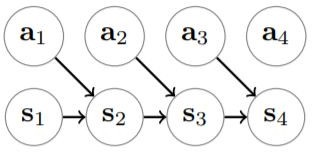
\includegraphics[width=0.85\linewidth,height=0.55\textheight,keepaspectratio]{images/soft-actor-critic/figures/mdp-graph.jpg}
        \caption*{Traditional Graph of MDP}
    \end{subfigure}\hfill
    \begin{subfigure}{0.45\textwidth}
        \centering
        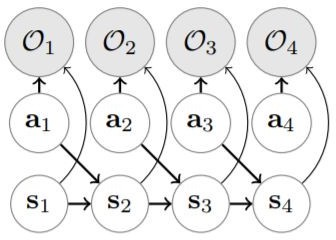
\includegraphics[width=0.95\linewidth,height=0.55\textheight,keepaspectratio]{images/soft-actor-critic/figures/optimality-graph.jpg}
        \caption*{Graphical Model with Optimality Variables}
    \end{subfigure}
\end{figure}
\end{frame}
\begin{frame}{Background: Control as Inference}
\textbf{Normal trajectory distribution}
\[
p(\tau) = p(\mathbf{s}_1, \mathbf{a}_1, \ldots, \mathbf{s}_T, \mathbf{a}_T \mid \theta) = p(\mathbf{s}_1) \prod_{t=1}^{T} p(\mathbf{a}_t \mid \mathbf{s}_t, \theta)\, p(\mathbf{s}_{t+1} \mid \mathbf{s}_t, \mathbf{a}_t).
\]

\textbf{Posterior trajectory distribution} \hfill $p(\mathcal{O}_t = 1 \mid \mathbf{s}_t, \mathbf{a}_t) = \exp(r(\mathbf{s}_t, \mathbf{a}_t))$.
\begin{align*}
p(\tau \mid \mathbf{o}_{1:T}) &\propto p(\tau, \mathbf{o}_{1:T}) = p(\mathbf{s}_1) \prod_{t=1}^{T} p(\mathcal{O}_t = 1 \mid \mathbf{s}_t, \mathbf{a}_t)\, p(\mathbf{s}_{t+1} \mid \mathbf{s}_t, \mathbf{a}_t) \\
&= p(\mathbf{s}_1) \prod_{t=1}^{T} \exp(r(\mathbf{s}_t, \mathbf{a}_t))\, p(\mathbf{s}_{t+1} \mid \mathbf{s}_t, \mathbf{a}_t) \\
&= \Bigg[ p(\mathbf{s}_1) \prod_{t=1}^{T} p(\mathbf{s}_{t+1} \mid \mathbf{s}_t, \mathbf{a}_t) \Bigg] \exp\!\left( \sum_{t=1}^{T} r(\mathbf{s}_t, \mathbf{a}_t) \right).
\end{align*}
\end{frame}
\begin{frame}{Background: Control as Inference}
\textbf{Variational Inference}
\begin{align*}
D_{\mathrm{KL}}(\hat{p}(\tau) \| p(\tau)) &= -\mathbb{E}_{\tau \sim \hat{p}(\tau)}[\log p(\tau) - \log \hat{p}(\tau)]. \\
-D_{\mathrm{KL}}(\hat{p}(\tau) \| p(\tau)) &= \mathbb{E}_{\tau \sim \hat{p}(\tau)}\Bigg[ \log p(\mathbf{s}_1) + \sum_{t=1}^{T} \Big( \log p(\mathbf{s}_{t+1} \mid \mathbf{s}_t, \mathbf{a}_t) + r(\mathbf{s}_t, \mathbf{a}_t) \Big) \\
&\qquad\qquad - \log p(\mathbf{s}_1) - \sum_{t=1}^{T} \Big( \log p(\mathbf{s}_{t+1} \mid \mathbf{s}_t, \mathbf{a}_t) + \log \pi(\mathbf{a}_t \mid \mathbf{s}_t) \Big) \Bigg] \\
&= \mathbb{E}_{\tau \sim \hat{p}(\tau)}\!\left[ \sum_{t=1}^{T} r(\mathbf{s}_t, \mathbf{a}_t) - \log \pi(\mathbf{a}_t \mid \mathbf{s}_t) \right] \\
&= \sum_{t=1}^{T} \mathbb{E}_{(\mathbf{s}_t, \mathbf{a}_t) \sim \hat{p}(\mathbf{s}_t, \mathbf{a}_t)}\!\left[ r(\mathbf{s}_t, \mathbf{a}_t) - \log \pi(\mathbf{a}_t \mid \mathbf{s}_t) \right] \\
&= \sum_{t=1}^{T} \mathbb{E}_{(\mathbf{s}_t, \mathbf{a}_t) \sim \hat{p}(\mathbf{s}_t, \mathbf{a}_t)}[r(\mathbf{s}_t, \mathbf{a}_t)] + \mathbb{E}_{\mathbf{s}_t \sim \hat{p}(\mathbf{s}_t)}[\mathcal{H}(\pi(\mathbf{a}_t \mid \mathbf{s}_t))].
\end{align*}
\end{frame}
